
Here, we describe prior reading time experiments and preregistrations.
We initially measured the effect of Embedding Bias in the \textsc{Three} condition (Section~\ref{sec:rt-three}--\ref{sec:rt-comp}).
We then preregistered theoretical predictions in the \textsc{Two} and \textsc{One} conditions for Embedding Bias and compatibility (Sections~\ref{sec:-rt-study-3}--\ref{sec:-rt-study-4}).
We then conducted a larger study examining all conditions, similar to Experiments 1 and 2 in the main paper, but with a partially different stimulus pool (Section~\ref{sec:-rt-study-5}).
We also report a meta-analysis that combines evidence from this study with Experiments 1--2 (Section~\ref{sec:meta}).

\subsection{Experiment S1: Reading Times in \textsc{Three}}\label{sec:rt-three}

We created 20 items and matched these randomly with 20 nouns for every participant.\footnote{Results are deposited in the project repository: \url{https://gitlab.com/m-hahn/resource-rational-surprisal/-/tree/main/experiments/maze/previous/study1_EmbeddingBias/Submiterator-master}.}
The items were derived from those used in the ratings studies described in Section~\ref{sec:ratings-studies}.
All trials were in the \textsc{Three} condition; no distinction was made based on semantic compatibility.
The same fillers were used as in Experiments 1--2, but the full pool was used for every participant as there were 20 (instead of 10 as in Experiments 1--2) critical trials per subject.

Unlike Experiments 1--2, sentences were aborted when the subject made a mistake; this means that data is only available for those critical trials to which subjects advanced successfully.
We recruited 124 self-declared English native speakers on Prolific.

The same exclusion criteria and data analysis were applied as in Experiments 1--2.
For the given design, the only fixed effects predictor was Embedding Bias.
Results are shown in Figure~\ref{fig:expt-s1}; they agree with the experiments described in the main paper, both in direction and size of the effect of Embedding Bias within \textsc{Three}.


\begin{figure}
	\centering

	\includegraphics[width=0.48\textwidth]{../resource-rational-surprisal/experiments/maze/previous/study1_EmbeddingBias/Submiterator-master/figures/rt-raw.pdf}
	\includegraphics[width=0.48\textwidth]{../resource-rational-surprisal/experiments/maze/previous/study1_EmbeddingBias/Submiterator-master/figures/posterior-histograms-main_effects.pdf}

	\caption{Experiment S1: Reading times within \textsc{Three} (N=124).  Left: Mean RTs per noun. Right: Posterior of embedding bias fixed effect in mixed-effects analysis of log-transformed RTs. }\label{fig:expt-s1}
\end{figure}

\subsection{Experiment S2: Reading Times in \textsc{Three}+\textsc{Compatible}}\label{sec:rt-comp}

This experiment was analogous to Experiment S2, but we changed the items so that the precritical verb phrase would be semantically compatible with the first noun.\footnote{Results are deposited in the project repository: \url{https://gitlab.com/m-hahn/resource-rational-surprisal/-/tree/main/experiments/maze/previous/study2_compatible/Submiterator-master}.}
We furthermore used a larger pool of 46 nouns, and constrained the matching of items and nouns as in Experiments 1--2.
Unlike Experiment S1, we used the Maze version with do-overs as used in Experiments 1--2.



We recruited 113 self-declared English speakers on Prolific.

Results are shown in Figure~\ref{fig:expt-s2}; they replicate those of Experiment S1 and agree with those of Experiments 1--2.


\begin{figure}
	\centering

	\includegraphics[width=0.48\textwidth]{../resource-rational-surprisal/experiments/maze/previous/study2_compatible/Submiterator-master/figures/rt-raw.pdf}
	\includegraphics[width=0.48\textwidth]{../resource-rational-surprisal/experiments/maze/previous/study2_compatible/Submiterator-master/figures/posterior-histograms-main_effects.pdf}

	\caption{Experiment S2: Reading times within \textsc{Three}+\textsc{Compatible} (N=113). Left: Mean RTs per noun. Right: Posterior of embedding bias fixed effect in mixed-effects analysis of log-transformed RTs. Note that measurement precision of per-noun means is reduced compared to other experiments because the number of nouns (46) is large, so that there are fewer data points per noun. However, the mixed-effects analysis shows strong evidence that the slope is negative, with a size agreeing with the other experiments.}\label{fig:expt-s2}
\end{figure}





\subsection{Experiment S3: Reading Times in \textsc{One} and \textsc{Two}}\label{sec:-rt-study-3}

We conducted a preregistered study of the effect of Embedding Bias in the \textsc{One} and \textsc{Two} conditions.
We preregistered the theoretical predictions at \url{https://aspredicted.org/822i4.pdf}.
For each subject, 5 trials were in the \textsc{One} condition and 5 trials in the \textsc{Two} condition.
We recruited 30 participants.


Stimuli, code, and data are deposited in the project repository\footnote{\url{https://gitlab.com/m-hahn/resource-rational-surprisal/-/tree/main/experiments/maze/previous/study3_OneTwo}}. 

The analysis included main effects of Embedding Bias and of the \textsc{Embedded} contrast (\textsc{Two} vs \textsc{One} contrast).
We conducted the same mixed-effects analysis as in Experiments 1--2.

Results are shown in Figure~\ref{fig:expt-s3}; they are consistent with those in Experiments 1--2.
Note that reading times are lower than in those experiments; this can be attributed to the fact that a larger fraction of stimuli in this early study had the frequent word \emph{was} as the critical word.



\begin{figure}
	\centering

	\begin{tabular}{cccc}
		\textbf{Reading Times}	& \textbf{Fixed Effects Estimates} \\
		\includegraphics[width=0.28\textwidth]{../resource-rational-surprisal/experiments/maze/previous/study3_OneTwo/Submiterator-master/figures/logRT-points-fit_NoLogTransform.pdf} &
	\includegraphics[width=0.48\textwidth]{../resource-rational-surprisal/experiments/maze/previous/study3_OneTwo/Submiterator-master/figures/posterior-histograms.pdf}
	\end{tabular}

	\caption{Experiment S3: Reading times in \textsc{One} and \textsc{Two} (N=30).}\label{fig:expt-s3}
\end{figure}




\subsection{Experiment S4: Effect of Compatibility on Reading Times}\label{sec:-rt-study-4}

Here, we report our initial study of the effect of Compatibility in the \textsc{Two} and \textsc{Three} conditions.
We preregistered the theoretical prediction at \url{https://aspredicted.org/88tk4.pdf}.
We preregistered investigating compatibility in both \textsc{Two} and \textsc{Three}, but, due to a scripting error, the experiment only had trials in the  \textsc{Two} condition and none in the \textsc{Three} condition.
The items were derived from those of the previous study.
As preregistered, we recruited 40 subjects.


Stimuli, code, and data are deposited in the project repository\footnote{\url{https://gitlab.com/m-hahn/resource-rational-surprisal/-/tree/main/experiments/maze/previous/study4_compatibility/}}.
Results are shown in Figure~\ref{fig:expt-s4}.
They are consistent with those in the main paper, but do not provide conclusive statistical evidence alone due to the small number of participants.

\begin{figure}
	\centering
	\begin{tabular}{cccc}
		\textbf{Reading Times}	& \textbf{Fixed Effects Estimates} \\
		\includegraphics[width=0.18\textwidth]{../resource-rational-surprisal/experiments/maze/previous/study4_compatibility/Submiterator-master/figures/logRT-points-fit_NoLogTransform.pdf} &
    \includegraphics[width=0.48\textwidth]{../resource-rational-surprisal/experiments/maze/previous/study4_compatibility/Submiterator-master/figures/posterior-histograms.pdf}
	\end{tabular}


	\caption{Results from Experiment S4 (N=40).}\label{fig:expt-s4}
\end{figure}

\subsection{Experiment S5: Large-Scale Replication of Experiments S3 and S4}\label{sec:-rt-study-5}

We next conducted a series of replications of Experiments S3 and S4, using larger sets of items (69) and nouns (40).
In particular, in addition to items from the previous experiments, 32 items were constructed specifically such that the  precritical word was constant across the \textsc{Compatible} and \textsc{Incompatible} conditions.
We recruited 431 subjects on Prolific.
This experiment consisted of multiple studies with successively larger pools of items that we analyze together here.
As in Experiments 1--2, there were 10 critical trials and 30 fillers per participant.

Stimuli, code, and data are deposited in the project repository\footnote{\url{https://gitlab.com/m-hahn/resource-rational-surprisal/-/tree/main/experiments/maze/previous/study5_replication}}. 


Experiments 1 and 2 in the main paper constitute replications of this study, but differ in that the stimulus pools were modified to avoid certain potential concerns regarding in the compatibility manipulation (see Section~\ref{sec:stimulus-pool}).


\begin{figure}
	\centering
	
	\begin{tabular}{cccc}
		\textbf{Reading Times}	& \multicolumn{2}{c}{\textbf{Fixed Effects Estimates}} \\
 &	Main Effects & Interactions \\
		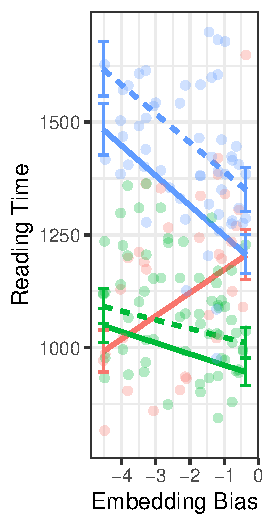
\includegraphics[width=0.2\textwidth]{../resource-rational-surprisal/experiments/maze/previous/study5_replication/Submiterator-master/figures/logRT-points-fit_errorbars_noLogTransform.pdf} &
		\includegraphics[width=0.35\textwidth]{../resource-rational-surprisal/experiments/maze/previous/study5_replication/Submiterator-master/figures/posterior-histograms-main_effects.pdf} &
	\includegraphics[width=0.35\textwidth]{../resource-rational-surprisal/experiments/maze/previous/study5_replication/Submiterator-master/figures/posterior-histograms-interactions.pdf}
	\end{tabular}



	\caption{Results from Experiment S5 (N=431). We show the posterior of the fixed effects in the mixed-effects model predicting log-transformed reading times (right), and reading times (left). As in Figure 3 in the main paper, we show empirical means per noun and condition, and mean reading times and standard deviations at ``fact''-like and ``report''-like nouns, all derived from the mixed-effects analysis. Results closely agree with those in Experiments 1--2, compare Figures~\ref{fig:expt1-fixed-effects}--\ref{fig:expt2-fixed-effects}.}\label{fig:expt5-results}
\end{figure}




We show reading time results in Figure~\ref{fig:expt5-results}.
Results agree closely with those of Experiments 1 and 2 (compare Figures~\ref{fig:expt1-fixed-effects}--\ref{fig:expt2-fixed-effects}).


\subsection{Meta-Analysis for Reading Time Studies}\label{sec:meta}

Here, we synthesize evidence from all large-sample reading time experiments covering \textsc{One}, \textsc{Two}, and \textsc{Three} (Study S5, Experiments 1--2), in order to provide as precise estimates of effect sizes as possible. 
High-precision estimates are useful both for comparison with theoretical models, and to inform future studies building on the effects reported in this paper.

There were a total of 119 items, including 32 appearing in Experiment 1, 42 items appearing in Experiment 2, and 45 items that only appeared in Study S5 and were not included in Experiments 1--2 (see Section~\ref{sec:stimulus-pool}).
The experiments had a total of 747 subjects, each with data from 10 critical trials.

Fixed-effects estimates and effects in raw reading times are shown in Figure~\ref{fig:meta}.
Estimates sharpen those from the individual experiments. In particular, effects of Embedding Bias and Compatibility are confirmed within both \textsc{Two} and \textsc{Three} individually:
\begin{enumerate}
	\item effect of depth $\widehat{\Delta} = 335$ ms, 95\% CrI $[294, 377]$, $Pr(\widehat{\Delta}<0) < 0.0001$
	\item Difference between `fact' and `report' in \textsc{One}: $\widehat{\Delta} = 222$  ms,   95\% CrI $[96 ,  347]$, $Pr(\widehat{\Delta}<0) < 0.0001$
	\item Difference between `fact' and `report' in \textsc{Two}: $\widehat{\Delta} = -89$   ms,  95\% CrI $[-146  , -33]$, $Pr(\widehat{\Delta}<0) = 0.004$
	\item Difference between `fact' and `report' in \textsc{Three}: $\widehat{\Delta} = -242$  ms,   95\% CrI $[-337,   -145]$, $Pr(\widehat{\Delta}<0) < 0.0001$
	\item Compatibility effect in \textsc{Two}: $\widehat{\Delta} = 39$ ms,   95\% CrI $[1  , 76]$,   $Pr(\widehat{\Delta}<0) =  0.02$
	\item Compatibility effect in \textsc{Three}:  $\widehat{\Delta} = 141$ ms   95\% CrI $[86,   198]$,    $Pr(\widehat{\Delta}<0) < 0.0001$
\end{enumerate}
Interactions \textsc{Depth}:\textsc{EmbeddingBias} and \textsc{Depth}:\textsc{Compatible} (Figure~\ref{fig:meta}) indicate that effects of Embedding Bias and Compatibility are stronger in \textsc{Three} than in \textsc{Two}, in agreement with model predictions at moderately high retention rates (Figure~\ref{fig:model-surprisal}).
This is also shown by the fact that the credible intervals for the effects in \textsc{Two} and \textsc{Three} are essentially disjoint.





\begin{figure}
	\centering


	\textbf{Fixed Effects Estimates}
	\begin{tabular}{cc}
	Main Effects & Interactions \\
		\includegraphics[width=0.48\textwidth]{../resource-rational-surprisal/experiments/maze/meta/figures/posterior-histograms-main_effects.pdf} &
	\includegraphics[width=0.48\textwidth]{../resource-rational-surprisal/experiments/maze/meta/figures/posterior-histograms-interactions.pdf}
	\end{tabular}

	\textbf{Effects in Raw Reading Times}

	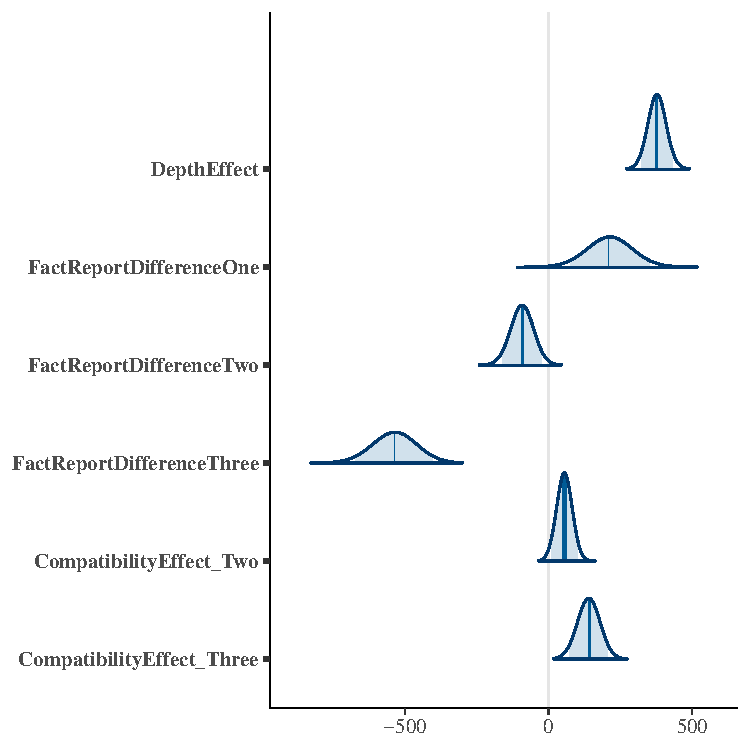
\includegraphics[width=0.48\textwidth]{../resource-rational-surprisal/experiments/maze/meta/figures/posterior-histograms-RawEffects.pdf}

	\caption{Results from meta-analysis ($N_{\text{subjects}}$=747, $N_{\text{items}}$=119). Top: Posteriors of fixed-effects coefficients for mixed-effects analysis of log-transformed reading times. Bottom: Effects transformed into raw reading times.}\label{fig:meta}
\end{figure}





\begin{figure}
	\centering


	\textbf{Fixed Effects Estimates}
	\begin{tabular}{cc}
	Main Effects & Interactions \\
		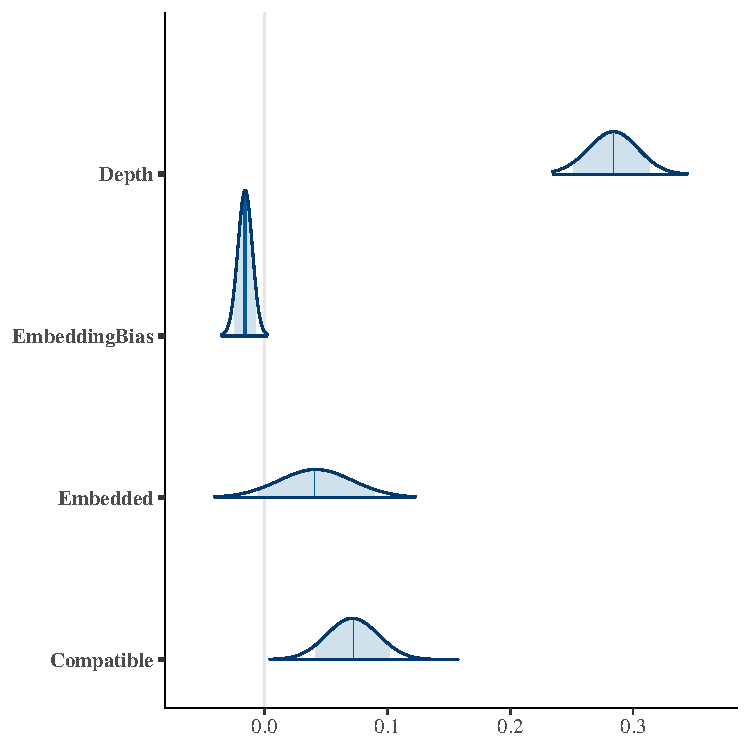
\includegraphics[width=0.48\textwidth]{../resource-rational-surprisal/experiments/maze/meta/figures/posterior-histograms-main_effects_prior.pdf} &
	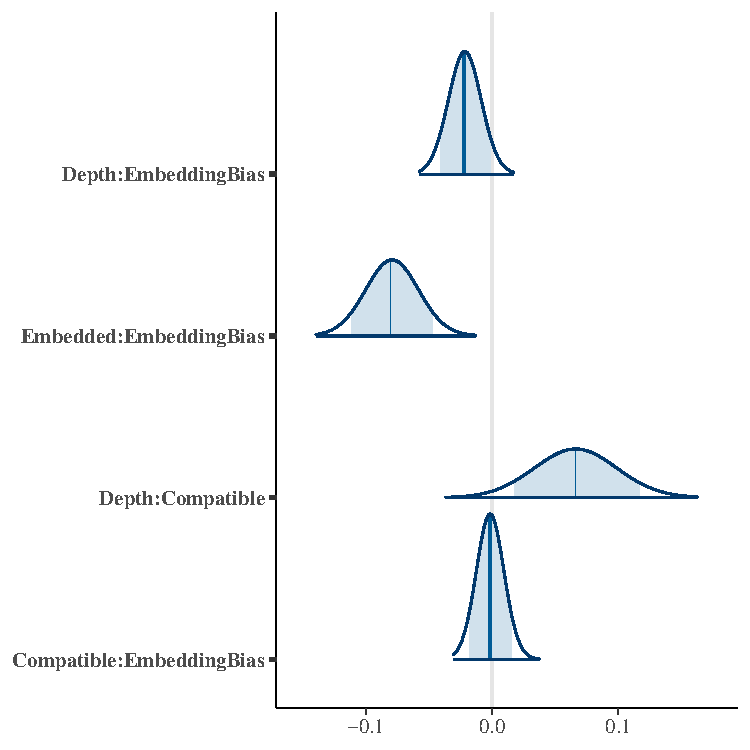
\includegraphics[width=0.48\textwidth]{../resource-rational-surprisal/experiments/maze/meta/figures/posterior-histograms-interactions_prior.pdf}
	\end{tabular}

	\textbf{Effects in Raw Reading Times}

	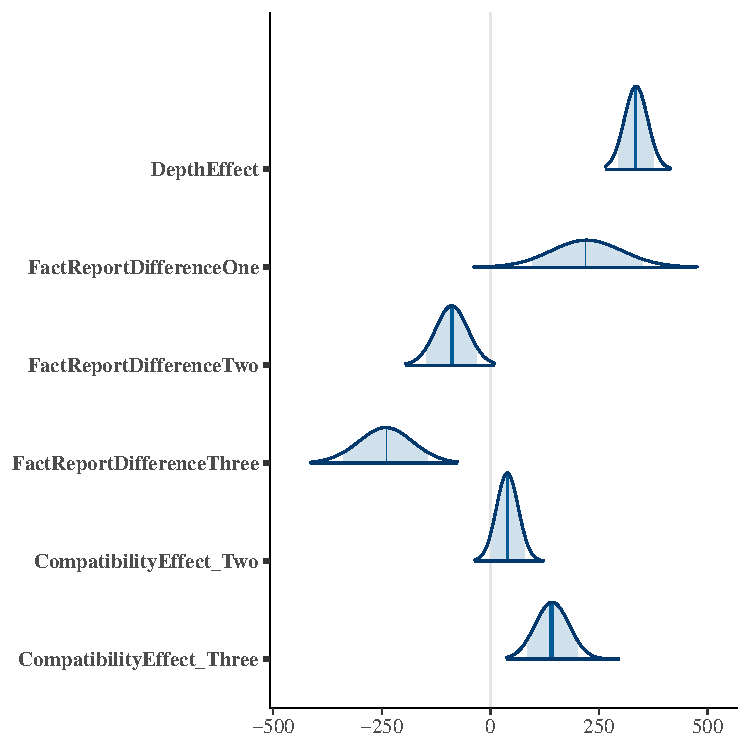
\includegraphics[width=0.48\textwidth]{../resource-rational-surprisal/experiments/maze/meta/figures/posterior-histograms-RawEffects_prior.pdf}

	\caption{Results from meta-analysis ($N_{\text{subjects}}$=747, $N_{\text{items}}$=119), analyzed with a mixed-effects analysis with a strongly regularizing prior $\mathcal{N}(0,1)$ for the fixed effects. The other parameters have the same prior as the analysis in Figure~\ref{fig:meta}: $t(3,7,2.5)$ for the intercept, $t(3,0,2.5)$ for the variance components, $LKJ(1)$ for the correlation matrices. Results are essentially identical to those in Figure~\ref{fig:meta}.}\label{fig:meta-regularizing}
\end{figure}





